% Created by tikzDevice version 0.6.2-92-0ad2792 on 2013-03-30 14:54:44
% !TEX encoding = UTF-8 Unicode
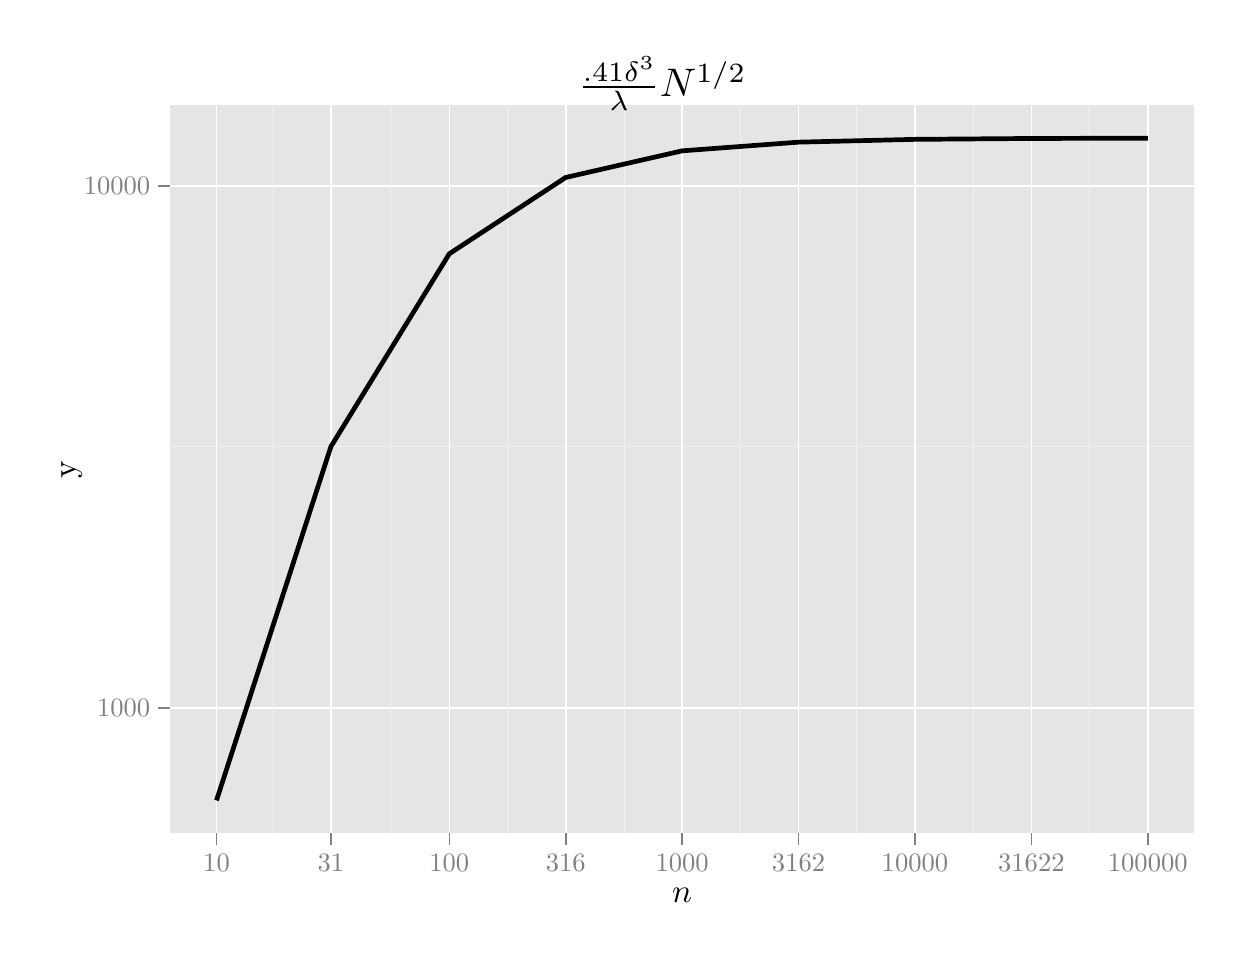
\begin{tikzpicture}[x=1pt,y=1pt]
\definecolor[named]{fillColor}{rgb}{1.00,1.00,1.00}
\path[use as bounding box,fill=fillColor,fill opacity=0.00] (0,0) rectangle (433.62,325.21);
\begin{scope}
\path[clip] (  0.00,  0.00) rectangle (433.62,325.21);
\definecolor[named]{drawColor}{rgb}{1.00,1.00,1.00}
\definecolor[named]{fillColor}{rgb}{1.00,1.00,1.00}

\path[draw=drawColor,line width= 0.6pt,line join=round,line cap=round,fill=fillColor] (  0.00,  0.00) rectangle (433.62,325.21);
\end{scope}
\begin{scope}
\path[clip] ( 51.42, 34.03) rectangle (421.57,297.23);
\definecolor[named]{fillColor}{rgb}{0.90,0.90,0.90}

\path[fill=fillColor] ( 51.42, 34.03) rectangle (421.57,297.23);
\definecolor[named]{drawColor}{rgb}{0.95,0.95,0.95}

\path[draw=drawColor,line width= 0.3pt,line join=round] ( 51.42,173.77) --
	(421.57,173.77);

\path[draw=drawColor,line width= 0.3pt,line join=round] ( 88.91, 34.03) --
	( 88.91,297.23);

\path[draw=drawColor,line width= 0.3pt,line join=round] (130.97, 34.03) --
	(130.97,297.23);

\path[draw=drawColor,line width= 0.3pt,line join=round] (173.39, 34.03) --
	(173.39,297.23);

\path[draw=drawColor,line width= 0.3pt,line join=round] (215.45, 34.03) --
	(215.45,297.23);

\path[draw=drawColor,line width= 0.3pt,line join=round] (257.53, 34.03) --
	(257.53,297.23);

\path[draw=drawColor,line width= 0.3pt,line join=round] (299.59, 34.03) --
	(299.59,297.23);

\path[draw=drawColor,line width= 0.3pt,line join=round] (341.65, 34.03) --
	(341.65,297.23);

\path[draw=drawColor,line width= 0.3pt,line join=round] (383.72, 34.03) --
	(383.72,297.23);
\definecolor[named]{drawColor}{rgb}{1.00,1.00,1.00}

\path[draw=drawColor,line width= 0.6pt,line join=round] ( 51.42, 79.46) --
	(421.57, 79.46);

\path[draw=drawColor,line width= 0.6pt,line join=round] ( 51.42,268.08) --
	(421.57,268.08);

\path[draw=drawColor,line width= 0.6pt,line join=round] ( 68.24, 34.03) --
	( 68.24,297.23);

\path[draw=drawColor,line width= 0.6pt,line join=round] (109.58, 34.03) --
	(109.58,297.23);

\path[draw=drawColor,line width= 0.6pt,line join=round] (152.37, 34.03) --
	(152.37,297.23);

\path[draw=drawColor,line width= 0.6pt,line join=round] (194.41, 34.03) --
	(194.41,297.23);

\path[draw=drawColor,line width= 0.6pt,line join=round] (236.50, 34.03) --
	(236.50,297.23);

\path[draw=drawColor,line width= 0.6pt,line join=round] (278.56, 34.03) --
	(278.56,297.23);

\path[draw=drawColor,line width= 0.6pt,line join=round] (320.62, 34.03) --
	(320.62,297.23);

\path[draw=drawColor,line width= 0.6pt,line join=round] (362.69, 34.03) --
	(362.69,297.23);

\path[draw=drawColor,line width= 0.6pt,line join=round] (404.75, 34.03) --
	(404.75,297.23);
\definecolor[named]{drawColor}{rgb}{0.00,0.00,0.00}

\path[draw=drawColor,line width= 1.7pt,line join=round] ( 68.24, 46.00) --
	(109.58,173.84) --
	(152.37,243.51) --
	(194.41,271.08) --
	(236.50,280.70) --
	(278.56,283.84) --
	(320.62,284.85) --
	(362.69,285.17) --
	(404.75,285.27);
\end{scope}
\begin{scope}
\path[clip] (  0.00,  0.00) rectangle (433.62,325.21);
\definecolor[named]{drawColor}{rgb}{0.50,0.50,0.50}

\node[text=drawColor,anchor=base east,inner sep=0pt, outer sep=0pt, scale=  0.96] at ( 44.30, 76.15) {1000};

\node[text=drawColor,anchor=base east,inner sep=0pt, outer sep=0pt, scale=  0.96] at ( 44.30,264.78) {10000};
\end{scope}
\begin{scope}
\path[clip] (  0.00,  0.00) rectangle (433.62,325.21);
\definecolor[named]{drawColor}{rgb}{0.50,0.50,0.50}

\path[draw=drawColor,line width= 0.6pt,line join=round] ( 47.15, 79.46) --
	( 51.42, 79.46);

\path[draw=drawColor,line width= 0.6pt,line join=round] ( 47.15,268.08) --
	( 51.42,268.08);
\end{scope}
\begin{scope}
\path[clip] (  0.00,  0.00) rectangle (433.62,325.21);
\definecolor[named]{drawColor}{rgb}{0.50,0.50,0.50}

\path[draw=drawColor,line width= 0.6pt,line join=round] ( 68.24, 29.77) --
	( 68.24, 34.03);

\path[draw=drawColor,line width= 0.6pt,line join=round] (109.58, 29.77) --
	(109.58, 34.03);

\path[draw=drawColor,line width= 0.6pt,line join=round] (152.37, 29.77) --
	(152.37, 34.03);

\path[draw=drawColor,line width= 0.6pt,line join=round] (194.41, 29.77) --
	(194.41, 34.03);

\path[draw=drawColor,line width= 0.6pt,line join=round] (236.50, 29.77) --
	(236.50, 34.03);

\path[draw=drawColor,line width= 0.6pt,line join=round] (278.56, 29.77) --
	(278.56, 34.03);

\path[draw=drawColor,line width= 0.6pt,line join=round] (320.62, 29.77) --
	(320.62, 34.03);

\path[draw=drawColor,line width= 0.6pt,line join=round] (362.69, 29.77) --
	(362.69, 34.03);

\path[draw=drawColor,line width= 0.6pt,line join=round] (404.75, 29.77) --
	(404.75, 34.03);
\end{scope}
\begin{scope}
\path[clip] (  0.00,  0.00) rectangle (433.62,325.21);
\definecolor[named]{drawColor}{rgb}{0.50,0.50,0.50}

\node[text=drawColor,anchor=base,inner sep=0pt, outer sep=0pt, scale=  0.96] at ( 68.24, 20.31) {10};

\node[text=drawColor,anchor=base,inner sep=0pt, outer sep=0pt, scale=  0.96] at (109.58, 20.31) {31};

\node[text=drawColor,anchor=base,inner sep=0pt, outer sep=0pt, scale=  0.96] at (152.37, 20.31) {100};

\node[text=drawColor,anchor=base,inner sep=0pt, outer sep=0pt, scale=  0.96] at (194.41, 20.31) {316};

\node[text=drawColor,anchor=base,inner sep=0pt, outer sep=0pt, scale=  0.96] at (236.50, 20.31) {1000};

\node[text=drawColor,anchor=base,inner sep=0pt, outer sep=0pt, scale=  0.96] at (278.56, 20.31) {3162};

\node[text=drawColor,anchor=base,inner sep=0pt, outer sep=0pt, scale=  0.96] at (320.62, 20.31) {10000};

\node[text=drawColor,anchor=base,inner sep=0pt, outer sep=0pt, scale=  0.96] at (362.69, 20.31) {31622};

\node[text=drawColor,anchor=base,inner sep=0pt, outer sep=0pt, scale=  0.96] at (404.75, 20.31) {100000};
\end{scope}
\begin{scope}
\path[clip] (  0.00,  0.00) rectangle (433.62,325.21);
\definecolor[named]{drawColor}{rgb}{0.00,0.00,0.00}

\node[text=drawColor,anchor=base,inner sep=0pt, outer sep=0pt, scale=  1.20] at (236.50,  9.03) {$n$};
\end{scope}
\begin{scope}
\path[clip] (  0.00,  0.00) rectangle (433.62,325.21);
\definecolor[named]{drawColor}{rgb}{0.00,0.00,0.00}

\node[text=drawColor,rotate= 90.00,anchor=base,inner sep=0pt, outer sep=0pt, scale=  1.20] at ( 17.30,165.63) {y};
\end{scope}
\begin{scope}
\path[clip] (  0.00,  0.00) rectangle (433.62,325.21);
\definecolor[named]{drawColor}{rgb}{0.00,0.00,0.00}

\node[text=drawColor,anchor=base,inner sep=0pt, outer sep=0pt, scale=  1.44] at (236.50,300.24) {$\frac{.41\delta^3}{\lambda}N^{1/2}\quad $};
\end{scope}
\end{tikzpicture}
